\chapter{跨域知识图谱的知识表示学习关键技术}
传统的知识图谱嵌入模型通过提取三元组中的事实特征来对实体和关系进行编码。这类模型设计了评分函数如TransE、RESCAL等对三元组进行打分。然而在跨域知识图谱的场景下,目标域知识图谱存在新的实体和关系,传统的嵌入模型不能很好地学习到这些实体和关系的表示。基于规则和归纳推理的方法从子图或关系结构中学习向量表示,未能充分利用知识图谱的语义信息。为了解决跨域知识表示问题,本文设计了一个基于本体信息和元学习的跨域知识表示学习模型。本章将介绍模型涉及到的本体嵌入方法、基于GNN的表示学习方法以及元学习相关的关键技术。

\section{跨域知识图谱的知识表示学习定义}
知识图谱由众多的事实三元组组成,通常可以被定义为\(\mathcal{G} = (\mathcal{E},\mathcal{R},\mathcal{T})\),其中\(\mathcal{E}\),\(\mathcal{R}\),\(\mathcal{T}\)分别指代图谱实体的集合、关系的集合和实体三元组的集合。事实三元组中头尾实体和关系分别来自于实体集\(\mathcal{E}\)和关系集\(\mathcal{R}\),即\(\mathcal{T}=\{(h,r,t) \subseteq \mathcal{E} \times \mathcal{R} \times \mathcal{E}\}\)。传统的知识图谱表示学习旨在将实体和关系映射到连续的低维向量空间,同时保留知识图谱的结构特征。为了验证知识表示学习的有效性,一般会评价其在下游任务的性能表现,并将三元组划分为用于模型参数学习的三元组\(\mathcal{T}_{support}\)及用于测试的三元组\(\mathcal{T}_{query}\)。如在尾结链接预测任务中,给定测试三元组中的一个事实\((h,r,t) \in \mathcal{T}_{query}\),通过模型计算其所有可能的候选三元组\(\{(h,r,e) | e \in \mathcal{E}, (h,r,e) \notin \mathcal{T}_{support} \cup \mathcal{T}_{query}\}\)的排名,在所有预测三元组中,事实三元组\((h,r,t)\)的排名越靠前,则表明该表示学习模型的效果越好。

在跨域知识图谱的现实场景中,需要将源知识图谱上训练的模型应用于目标知识图谱上。由于成本、用户数据隐私等限制,无法将目标知识图谱与源知识图谱合并后重新训练,因此划分出跨域知识图谱。其中\(\textbf{源域知识图谱}\)包含大量已知事实三元组用于训练,\(\textbf{目标域知识图谱}\)作为源域知识图谱子集可能包含未定义的实体和关系用于测试。现给定一个用于训练的源域知识图谱\(\mathcal{G}^{train} = (\mathcal{E}^{train})\),并以在源域知识图谱上进行模型参数的学习为目标任务,从而能够将该模型应用在包含未见实体和未见关系的目标域知识图谱上,即\(\mathcal{G}^{test} = (\mathcal{E}^{test},\mathcal{R}^{test},\mathcal{T}^{test}_{support},\mathcal{T}^{test}_{query})\)。跨域知识图谱中的实体集和关系集遵循\((\mathcal{E}^{train} \neq \mathcal{E}^{test},\mathcal{E}^{train} \cap \mathcal{E}^{test} \neq \emptyset)\)及\((\mathcal{R}^{train} \neq \mathcal{R}^{test},\mathcal{R}^{train} \cap \mathcal{R}^{test} \neq \emptyset)\)。其中\(\mathcal{T}^{test}_{support}\)只用于标记测试集中实体与关系的结构,不用于对模型的训练。
\section{本体嵌入关键技术}
本体图是一种特殊的知识图谱,本体规定了一系列基本概念之间的语义关系。通常本体以层次概念为主干,通过属性来描述概念的语义关系,以表示通用或特定领域的知识。随着知识表示学习的不断发展,传统基于三元组结构信息进行表示学习的方法在面对跨域知识图谱等场景下,存在一定局限性。因此,越来越多的方法尝试引入本体信息,以提高表示学习的效果。如图\ref{fig:2-1}所示,这些本体信息不仅描述实体或关系的限制条件,如属性域和取值范围等,也是对知识图谱语义信息的抽象和集中表示。
\begin{figure}[h]
  \centering
  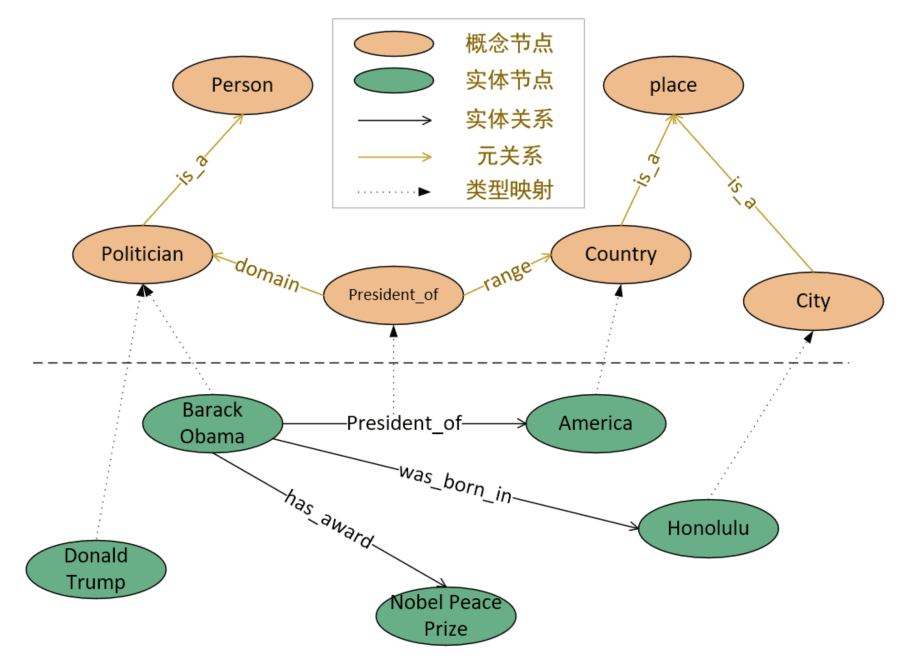
\includegraphics[width=0.8\textwidth]{2-1.png}
  \caption{知识图谱的本体视角和实例视角}
  \label{fig:2-1}
\end{figure}

本体图包含概念和概念间的元关系,通常被定义为\(\mathcal{G} = (\mathcal{C},\mathcal{P})\),其中\(\mathcal{C}\)是概念的集合,\(\mathcal{P}\)是元关系的集合。类似于实体三元组,一个本体三元组(s,r,t)表示概念s,t通过元关系r进行联系。然而,与实例知识图谱复杂多样的关系不同,元关系可进一步分类为传递关系、对称关系、层次关系和其他简单关系\cite{chen2018on2vec}。受KGE方法的启发,On2Vec\cite{chen2018on2vec}尝试将本体概念和元关系映射为低维向量。但该模型认为本体关系大多具有传递、对称等特性,不能直接将KGE方法应用在本体图上。例如对称关系r的两个三元组(c$_{1}$,r,c$_{1}$)和(c$_{1}$,r,c$_{1}$),当采用TransE等方法学习嵌入时,无法同时兼顾三元组对应的向量满足\(\textbf{c}_{1,r} + \textbf{r} ≈ \textbf{c}_{2,r}\)和\(\textbf{c}_{2,r} + \textbf{r} ≈ \textbf{c}_{1,r}\)。为了解决上述问题,On2Vec通过设置两个关系特定的投影函数,来区分同一概念在特定关系头尾位置的不同编码,如公式\ref{eq:2-1}所示:
\begin{equation}
  S_{d}(T) = || f_{1,r}(\textbf{s}) + \textbf{r} -f_{2,r}(\textbf{t})||,\label{eq:2-1}
\end{equation}
其中\(f_{1,r}\)和\(f_{2,r}\)分别代表了对特定关系r的三元组作为头本体和尾本体不同的投影操作。通过对头部本体和尾部本体分别进行不同的投影,可以解决上述传递元关系和对称元关系引起的矛盾问题。对于头尾本体投影操作的选择,On2Vec采用了简单的线性变换处理,如公式\ref{eq:2-2}所示:
\begin{equation}
  \begin{aligned} 
    &f_{1,r}(\textbf{s}) = \textbf{M}_{1,r}\textbf{s}, \quad\textbf{M}_{1,r} \in \mathbb{R}^{k \times k}, \\
    &f_{2,r}(\textbf{s}) = \textbf{M}_{2,r}\textbf{s}, \quad\textbf{M}_{2,r} \in \mathbb{R}^{k \times k},
    \end{aligned} \label{eq:2-2}
\end{equation}

特别对于层次关系,On2Vec将层次关系进一步划分为R$_{r}$和R$_{c}$,R$_{r}$表示粗略概念被划分为更细致概念的细化关系,而R$_{c}$表示将更细致概念分组为更粗略概念的简略关系。该模型为使细致概念的嵌入汇聚在一个更紧密的邻域内,采用层次模型对层次关系进行单独的处理。对层次关系嵌入的评分函数设置如公式\ref{eq:2-3}所示:
\begin{equation}
  \begin{aligned} 
    S_{hm}(G) = &\sum_{r\in R_{r}} \sum_{s\in C} \sum_{r\in \sigma(s,r)} \omega(f_{1,r}(\textbf{s}) + \textbf{r},f_{2,r}(\textbf{t}))\\
    + &\sum_{r\in R_{c}} \sum_{t\in C} \sum_{r\in \sigma(t,r)} \omega(f_{2,r}(\textbf{t}) -\textbf{r},f_{1,r}(\textbf{s})),
    \end{aligned} \label{eq:2-3}
\end{equation}
其中,\(\omega\)为两个参数向量的角度或距离单调递增的函数,On2Vec采用余弦距离函数。\(\sigma\)为对相应层次关系的本体节点的搜索操作,包括对细化关系寻找所有该关系下的所有尾本体、对简略关系寻找该关系下的所有头本体。On2Vec扩展了TransE方法,通过捕获本体关系的关系属性和层次结构,实现了对本体概念和元关系的表示,同时证明了在本体图上应用知识图谱嵌入方法的有效性。

现有的大多数本体模型在知识嵌入过程中都只包含单一的本体信息,对表示学习的补充作用有限,如SSE\cite{guo2016sse}、TKRL\cite{xie2016representation-TKRL}都仅采用了本体中实体类型信息,无法实现对所有可用本体信息的嵌入。本文能够在知识嵌入过程中整合所有可用的本体信息,充分补充图谱,提高复杂场景下的决策能力。同时本文使用了一种简单的本体形式,即RDF模式(RDF Schema,RDFS),而那些更复杂的OWL本体可以按照一定的标准转换为RDFS本体。

\section{基于GNN的跨域知识表示学习关键技术}
图神经网络模型是专门用于处理图数据的模型,对图结构进行编码,并进行节点级别、边级别及图级别的预测任务。CNN模型只能作用在具有相同结构的图像或者特定序列的语音和文字上,而图数据没有固定的形式且邻居节点也都是无序的,因此CNN模型无法作用在复杂的知识图谱上。相比之下,GNN通过聚合和更新操作,能够学习到图谱结构和节点特征的有效信息。

为学习到图的结构信息和节点特征,GNN主要包含了两个部分:聚合函数和更新函数。聚合函数可以将相邻节点的特征进行聚合,可以使用诸如sum、mean和max等聚合操作。一次聚合操作可以提取邻接节点的信息,这些邻接节点距离当前节点为一跳。GNN通常包含多层,每一层都会用上一层的信息进行聚合和传递。因此,n层聚合后传递的信息包含了n层邻接节点的结构信息和节点本身的特征信息。每层的特征聚合函数,如公式\ref{eq:2-7}所示:
\begin{equation}
  h_{v}^{k} = \sigma(W_{k} \sum \frac{h_{u}^{k-1}}{|N(v)|} + B_{k}h_{v}^{k-1}) \quad where \quad k = 1, ..., k-1 \label{eq:2-7}
\end{equation}
其中本层输出特征\(h_{v}^{k}\)包含两个组成部分。\(W_{k}\sum\frac{h^{k-1}_{u}}{|N(v)|}\)表示邻接点特征的聚合操作,后一部分是上一层聚合的特征与本层权重参数的乘积。这两部分特征通过激活函数更新,输出本层节点的特征表示。在GNN模型中,聚合函数没有区分邻接节点的重要性,仅采用简单的池化操作。

基于GNN的一种改进方向为集中于对图中关系表示的补充。图神经网络关注节点特征的聚合和更新操作,但在信息传递的过程中,图的关系结构仅用于指明邻接点,关系特征未参与节点的更新过程。为了增加关系信息对节点的影响,R-GCN在每层节点特征计算中引入了邻接点间的对应关系,更新函数如公式\ref{eq:2-8}所示:
\begin{equation}
  h_{i}^{l+1} = \sigma \left( \sum_{r\in\mathcal{R}} \sum_{j\in\mathcal{N}_{i}^{r}} \frac{1}{c_{i,r}}W_{r}^{l}h_{j}^{l} + W_{0}^{l}h_{i}^{l}\right), \label{eq:2-8}
\end{equation}

与GNN对邻接点特征聚合的操作不同,R-GCN引入了关系特定的转换。这种转换取决于边的类型和方向。为确保第l层的节点表示可以受到自身层次表示的影响,R-GCN在基础的图关系上为每个节点添加了一个自连接的特殊关系。如图\ref{fig:2-2}所示,在R-GCN中每层对一个实体节点(红色块表示)进行特征生成的过程中,首先从邻接点获取特征(蓝色块表示)并根据该节点与邻接节点的关系类型进行特征转换得到该种关系对应的表示(绿色块表示),其中关系类型分别由入关系、出关系以及自循环关系组成。然后将所有根据关系类型转换后的邻接节点信息累加求和,并通过一个如ReLU的激活函数更新,即可获得该节点本层的输出表示。相比于R-GCN,近期提出的CompGCN在R-GCN模型的基础上进一步引入了注意力机制,针对每种边类型和方向分别进行了注意力计算以加强对重要信息的关注。而且在计算效率方面,它减少了每个节点的嵌入大小及依赖于固定卷积核的计算量,因此更适合于大规模图数据。
\begin{figure}[h]
  \centering
  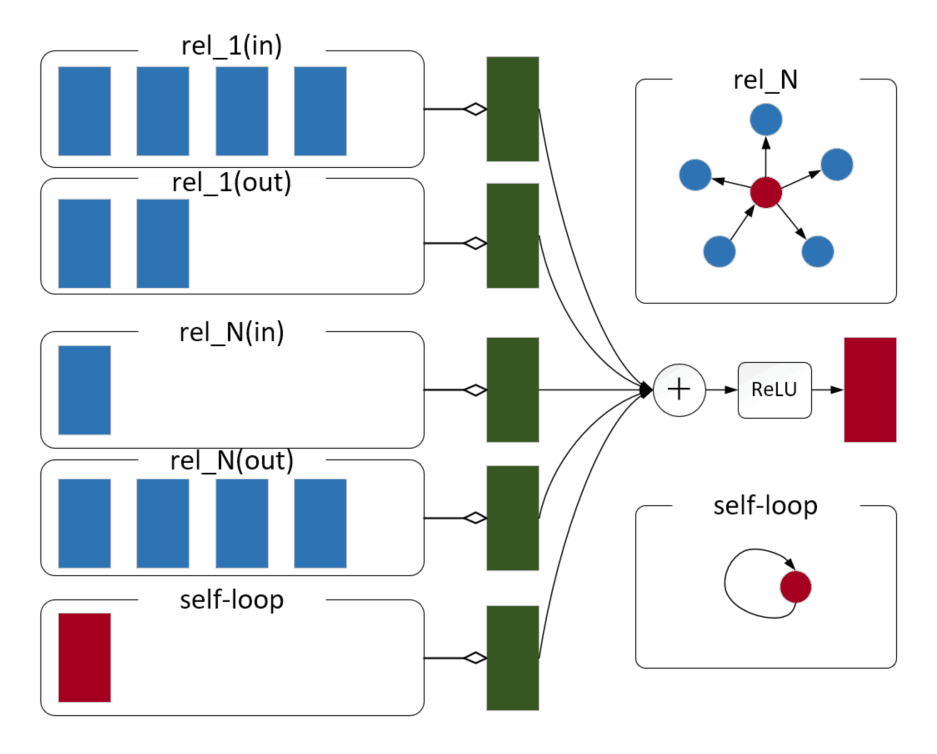
\includegraphics[width=0.7\textwidth]{2-2.png}
  \caption{R-GCN的特征传递}
  \label{fig:2-2}
\end{figure}

图神经网络通过聚合实体的邻域信息进行表示学习,一定程度上已经可以处理跨域知识表示问题,许多方法将GNN与其他方法结合进一步加强跨域知识表示学习效果。例如,INDIGO\cite{liu2021indigo}模型使用实体三元组与GNN的内层和外层的特征向量元素之间的一一对应关系对知识图谱进行编码,并避免了额外的打分函数,充分利用了GNN的特征聚合能力。其他方法如Zhao\cite{zhao2020attention}等人通过基于注意力的图网络聚合未见关系的邻接结构特征,来作为未见关系的表示。但这些方法要么专注于传统的知识表示学习领域,要么通过结构信息对未见的实体或关系进行嵌入,忽略了图谱的语义信息。本文通过全局本体信息的嵌入表示,在加强知识引入的同时,借助关系的位置结构信息来训练一个兼顾未见实体和关系的基于GNN的表示学习模型。

\section{元学习训练方法}
元学习最普适性的算法思想可以理解为“learning to learn”,它通过多个学习任务的训练来改进学习算法,而传统的机器学习算法则是在多个数据实例上进行模型的学习。

传统的机器学习方法会设置一个训练集\(\mathcal{D} = \{(x_{1},y_{1}),...,(x_{N},y_{N})\}\),如样本对(输入的图片,图片的标签)。而元学习的目的是训练出一个模型函数\(y = f_{\theta}(x)\),通过训练来获得其中的参数\(\theta\),求解公式如公式\ref{eq:2-9}所示:
\begin{equation}
  \theta^{*} = \underset { \theta } { \operatorname { arg } \operatorname { min } }\mathcal{L}(\mathcal{D};\theta,\omega) \label{eq:2-9}
\end{equation}
其中的\(\mathcal{L}\)是一个用于计算真实标签与模型预测标签之间的误差的损失函数,\(\omega\)指代了模型如何学习的假设,例如如何为参数\(\theta\)选择合适的优化器或者为\(f\)选择函数类型等。传统的机器学习方法实现过程中,该部分由研究者手动设置。模型的泛化性能则通过评估模型在已知标签测试集上的任务性能来衡量。传统的机器学习假设模型的优化在每个训练集\(\mathcal{D}\)上由初始参数开始执行,模型如何学习的设定是预先指定的,而这些设定将极大地影响模型的准确性和数据效率等性能指标。元学习试图从任务中通过学习学习算法本身来改进这些指标,而不是假设学习算法是预先指定或者固定的。

元学习可以视为一个双层优化问题,其中包含内外两层。双层优化\cite{stackelberg1952theory}是指一类层次性优化问题,其中一个优化问题包含另一个优化问题作为约束\cite{franceschi2018bilevel}\cite{sinha2017review}。经典的内外双层模型的算法如MAML,其算法流程如算法\ref{alg:meta}所示:
\begin{algorithm}
  \KwData{\(p(\mathcal{T})\):distribution over tasks}
  \KwData{\(\alpha,\beta\) step size hyperparameters}
    randomly initialize \(\theta\) \\
    \While{not done}{
    Sample batch of tasks \(\mathcal{T}_{i} \thicksim p(\mathcal{T})\)
    \For{\(\mathcal{T}_{i}\)}{
      Evaluate \(\nabla_{\theta}\mathcal{L}_{\mathcal{T}_{i}}(f_{\theta})\) wtih respect to K examples \\
      Compute adapted parameters with gradient descent:\(\theta^{'}_{i} = \theta - \alpha\nabla_{\theta}\mathcal{L}_{\mathcal{T}_{i}}(f_{\theta})\)
    }
    Update \(\theta \leftarrow \theta - \beta\nabla_{\theta} \sum_{\mathcal{T}_{i} \thicksim p(\mathcal{T})}\mathcal{L}_{\mathcal{T}_{i}}(f_{\theta^{'}})\)
  }
  \caption{MAML模型算法流程}\label{alg:meta}
  \end{algorithm}

  在该视角下,元学习任务可以通过公式\ref{eq:2-10}所示来规范化:
\begin{equation}
  \omega ^ { * } = \underset { \omega } { \operatorname { arg } \operatorname { min } } \sum_{i=1}^{M} \mathcal{L} ^ { \text { meta } } ( \mathcal{D} _ { \text { source } } ^ { \text { val } ( i ) } ; \theta ^ { * ( i ) } , \omega ), \label{eq:2-10}
\end{equation}
\begin{equation}
  s.t. \qquad \theta ^ { * ( i ) } ( \omega ) = \underset { \theta } { \operatorname { arg } \operatorname { min } } \mathcal{L} ^ { \text { task } } ( \mathcal{D} _ { \text { source } } ^ { \text { train } ( i ) } ; \theta , \omega ), \label{eq:2-11}
\end{equation}
其中\(\mathcal{L} ^ { \text { meta } }\)和\(\mathcal{L} ^ { \text { task } }\)分别指代外层的优化目标和内层的优化目标,如在分类任务下的交叉熵。但是这两层的优化级别并不对称,内层优化在基于外层参数\(\omega\)的优化过程中不能对\(\omega\)进行修改。公式中\(\omega\)可以指代如非凸优化\cite{finn2017model}的内层模型的初始化参数或其他可学习的超参数。因此,元学习的整个模型训练分为了两层:内层模型首先接收外层模型的参数\(\omega\),然后根据自己的任务在该任务的训练集上进行训练,并在任务的测试集上计算出损失;外层模型接收内层模型计算出的损失,并对参数\(\omega\)进行更新,使得内层函数的损失趋向最优。元学习的思想即通过外层模型的训练,学习到内层模型一个较优的设定,可以让内层模型更好的完成其他任务。

如前所述,内层模型在训练的时候需要针对面向的问题提供相应的训练集和测试集,这里以任务为训练单位的设定也是元学习方法区别于传统机器学习方法的一大特点。从训练任务的角度而言,元学习的目标即学习一种通用的、能够作用在各任务上的学习算法,这些学习到的算法能够在新的任务上获得更好的表现效果。内层模型可以视为带有外层模型参数\(\omega\)的传统机器学习算法,其数据集为\(\mathcal{D} = (\mathcal{D}^{train}, \mathcal{D}^{val})\),针对单个任务的损失函数为\(\mathcal{L}(\mathcal{D};\omega) = \mathcal{L}(\mathcal{D}^{val};\omega^{*}(\mathcal{D}^{train},\omega),\omega)\)。在实际应用中,通常只有一个训练集和测试集。因此,一般会从源训练集中抽样出一组任务用于训练。这些任务的训练集和测试集被称为support集和query集,以避免与最终模型训练后进行评估的测试集混淆。

本文旨在进行跨域知识图谱上进行知识表示的相关研究,并在含有未见实体和关系的目标域知识图谱上的链接预测任务上进行模型效果评估。传统的知识图谱表示学习的链接预测任务采用的数据集通常包含一个训练集和测试集,测试集中不包含新的实体和关系。因此,本文从现有数据集中构建符合跨域场景的测试集,并借鉴元学习“learning to learn”的思想,从训练数据中抽取多个任务用于训练,从任务上学习到对未见实体和关系的表示能力。

\section{本章小结}
本章首先介绍了跨域知识图谱的知识表示学习的定义,强调了跨域知识表示学习中新的实体和关系对传统知识表示学习的影响。对于如何将本体信息用于到知识表示中,介绍了使用本体嵌入的基本方法和代表性的一些应用模型。本体的向量表示,能够为实例图谱的实体和关系提供较为完整的语义信息。同时,本文结合GNN模型对邻接实体和关系的特征进行学习,在第三部分介绍了GNN在知识图谱的知识表示学习上的应用及基于GNN改进的一些模型方法。最后介绍了元学习相关的思想、原理及方法,为后续模型的任务划分及训练流程提供理论支撑和参考。